\chapter{L'outil de manipulation de texte rêvé}

Alors oui, pour ceux qui se demandent, je fais des rêves bizarres, mais bon chacun a ses petites tares cachées. Et rêver d'un outil qui améliore ma vie quotidienne en tant que codeur (ou écrivain, ou formateur, ou \ldots) n'est pas si étrange que ça.

Ce qui fait et fera encore le succès de \vim est sa capacité à \textbf{faciliter les manipulations de texte}. Certes il va vous proposer des fonctionnalités propres à chaque tâche que vous effectuerez \footnote{Souvent par l'intermédiaire de plugins.} comme la validation syntaxique de code, la correction orthographique, \ldots Mais à la fin, c'est toujours à écrire/corriger/manipuler/se déplacer dans du texte que vous passerez la majeure partie de votre temps. 

C'est là que l'approche de \vim est différente d'IDE comme Eclipse / Netbeans / PhpStorm et consorts. Là où ces IDE vont mettre l'accent sur les particularités de votre langage de programmation tout en vous fournissant des capacités de manipulation de texte basiques, \vim adopte l'approche opposée : vous serez \textbf{très efficace} à manipuler/écrire du texte quel que soit le texte et vous pourrez enrichir \vim avec des fonctionnalités propres à votre langage de programmation via des plugins.

Nous allons donc voir dans ce chapitre comment utiliser \vim à bon escient (vous allez commencer à oublier votre souris) et quelle est la logique derrière tous ces enchaînements de commandes qui paraissent barbares au non-initié. Vous devriez pouvoir, à la fin de ce chapitre, \textbf{vous passer de votre souris} pour éditer/manipuler le contenu d'un fichier\footnote{En tout cas, vous devriez vous forcer à le faire en apprenant \vim, ce n'est pas si dur que ça, et c'est ce qui fait la différence entre \vim et les autres : le tout clavier.}.

\section{Se déplacer par l'exemple : Essayer de copier / coller}\label{sec:se-deplacer}


Nous avons déjà vu dans la section «\nameref{sec:modeinsertion}» comment passer du mode insertion (pour saisir du texte) au mode normal (\emph{a priori} pour l'instant, vous ne savez pas trop à quoi sert ce mode). En appuyant sur \tti votre curseur passe en mode insertion (lorsque vous êtes en mode normal) et en appuyant sur \ttesc il repasse dans le mode normal. Bon bah on est bien Tintin. Et maintenant ? 

\subsection{Préambule}

Nous allons apprendre notre première manipulation de texte : le copier / coller. J'en vois certains d'entre vous se dire que ça ne sert à rien, car vous savez déjà le faire. Vous passez en mode insertion, vous prenez votre souris (ou vous vous déplacez avec les flèches directionnelles tout en appuyant sur \ttshift) pour sélectionner du texte et vous allez dans le \Verb|menu Édition| puis \Verb|Copier|. Et ensuite \Verb|menu Édition| puis \Verb|Coller|. Bah tiens, essayez pour voir.

Si vous avez suivi la section «\nameref{sec:modes}» traitant de la position idéale pour vos mains, vous savez que vous avez fait une ou plusieurs choses que vous devriez vous interdire :


\begin{itemize}
    \item Vous avez utilisé votre souris
    \item Vous avez déplacé grandement votre main droite de sa position de repos, pour aller atteindre les flèches directionnelles qui sont très mal placées sur un clavier
\end{itemize}


Alors certes ce n'est pas grave en soi, mais c'est \textbf{inefficace} (se servir de la souris ou déplacer votre main droite vers les touches directionnelles est très lent) et \textbf{nuisible} pour vos petites mains. Ceci est votre dernière chance : si vous n'êtes pas prêt à vous forcer à ne pas le faire, \textbf{\vim n'est pas fait pour vous}. \vim est parfait pour ne pas utiliser la souris et pour ne pas bouger vos mains (ou presque). Ne pas se forcer à le faire, c'est ne pas tirer tout le potentiel de \vim, et à un moment ou un autre, \textbf{vous le quitterez pour un éditeur} qui aura été pensé pour être utilisé à la souris. Alors, on continue ?

\subsection{Se passer de la souris}

Si vous lisez ces lignes c'est que vous avez répondu «oui», allons-y gaiement alors ! Nous allons tout d'abord commencer par nous passer de la souris. La prochaine étape sera de se passer des touches directionnelles, mais chaque chose en son temps.


\newthought{Pour réaliser un copier/coller} avec \vim tout se passe en mode «normal». Pour savoir dans quel mode vous vous trouvez, vous avez juste à regarder en bas à gauche de votre \vim. La figure \ref{fig:insert} vous montre \vim en mode «insertion» par exemple. Lorsque rien n'est marqué en bas à gauche, c'est que vous êtes en mode normal. Pour sortir d'un mode afin de retourner au mode normal, il suffit d'appuyer sur \ttesc\footnote{Si vous vous demandez pourquoi je vous dis d'arrêter d'utiliser la souris et/ou les touches directionnelles, mais que je ne dis rien sur le fait qu'il faille se torturer la main pour atteindre \ttesc, c'est que vous êtes sur la bonne voie. Je vous explique le comment du pourquoi dans «\nameref{sec:esc}».}.

\begin{figure}%
  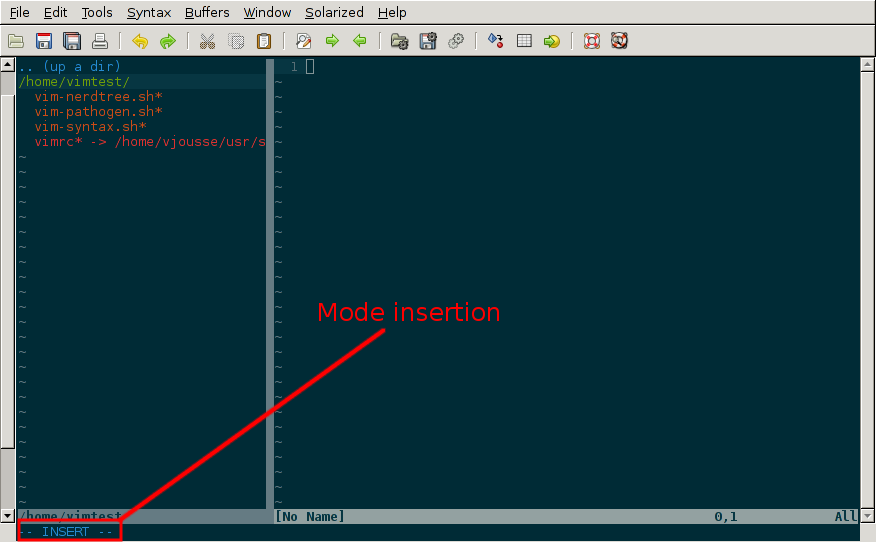
\includegraphics[width=\linewidth]{vim-insert.png}
  \caption{\vim en mode insertion.}
  \label{fig:insert}
\end{figure}

Admettons donc que vous êtes en mode «normal» et que vous avez un peu de texte de saisi dans votre \vim. Par exemple, cette chouette citation de Mark Twain : «Ils ne savaient que c'était impossible, alors ils l'ont fait.». Votre \vim devrait ressembler à celui de la figure \ref{fig:vim-twain}\footnote{Notez l'absence d'affichage d'un quelconque mode en bas à gauche.}.

\begin{figure}%
  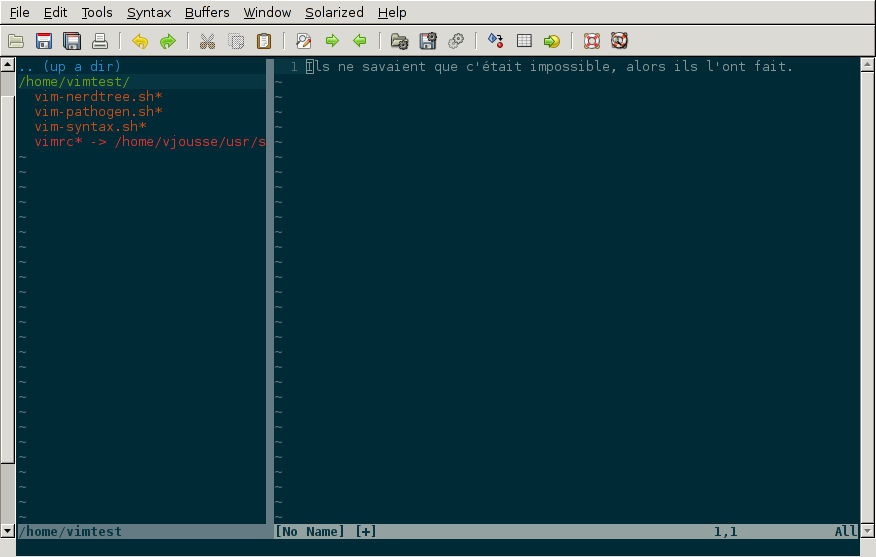
\includegraphics[width=\linewidth]{vim-twain.png}
  \caption{\vim prêt pour le copier/coller.}
  \label{fig:vim-twain}
\end{figure}

La façon la plus naturelle\footnote{Mais pas la plus efficace, nous verrons cela un peu plus loin.} de copier/coller le mot «impossible» va être de se déplacer sur la première lettre du mot avec les touches directionnelles, d'appuyer sur \ttv (pour passer en mode «visuel»), de se déplacer sur la dernière lettre (vous devriez avoir le mot sélectionné, en surbrillance) puis d'appuyer sur \tty\footnote{La touche \ty étant utilisée comme raccourci du mot \emph{yank} en anglais.}. Vous avez copié votre premier mot.

Déplacez vous ensuite à la fin de la phrase (toujours en mode «normal») puis appuyez sur \ttp\footnote{Raccourci du mot \emph{paste} cette fois ci.}. Le mot devrait avoir été collé à la fin, et vous devriez avoir le même rendu que la figure \ref{fig:vim-paste}.

\begin{figure}%
  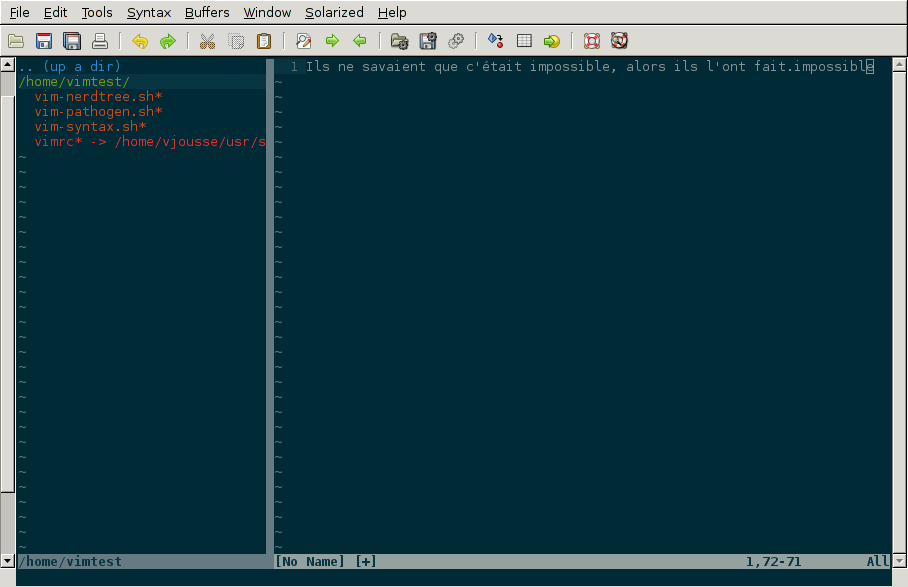
\includegraphics[width=\linewidth]{vim-paste.png}
  \caption{\vim après le copier/coller.}
  \label{fig:vim-paste}
\end{figure}

On se rend donc compte ici que \vim se sert de l'astuce des modes (et notamment du mode «normal» pour les déplacements) afin de ne pas avoir à se servir de la souris.
À partir du moment où vous aurez pris l'habitude de passer rapidement d'un mode à l'autre (et pour cela se passer de \ttesc va devenir indispensable), utiliser la souris vous apparaîtra comme une perte de temps, mais pour cela il va falloir pratiquer un peu bien sûr.


\section{Se passer des touches directionnelles}

Nous y voilà. Encore plus que de se priver de la souris, se priver des touches directionnelles est la chose à faire si l'on veut utiliser \vim, pour de vrai. \vim va vous permettre de faire tout plus rapidement et plus intuitivement à la seule condition de le faire sans les touches directionnelles.
Cela va vous permettre comme je l'ai déjà dit de ne pas bouger votre main certes, mais ça va aussi vous forcer à passer en mode «normal» pour réaliser vos déplacements et vos mouvements de texte. Il n'y a qu'à ce moment là\footnote{Un peu douloureux au début il est vrai.} que vous commencerez à vraiment tirer parti de \vim.

Pour cette section, je vais vous expliquer comment vous déplacer sans utiliser les touches directionnelles. Puis, une fois que vous aurez une vague idée de comment faire, je vous donnerai le code à mettre dans votre \vimrc pour désactiver les touches directionnelles complètement. Car oui, il n'y a que comme ça que vous y arriverez (en tout cas il n'y a que comme ça que j'y suis arrivé).


\subsection{Se déplacer}

En mode normal, 4 touches vont vous permettre de déplacer le curseur d'un caractère :
\begin{itemize}
    \item \tth pour aller à gauche
    \item \ttj pour aller en bas
    \item \ttk pour aller en haut
    \item \ttl pour aller à droite
\end{itemize}

\begin{figure}%
  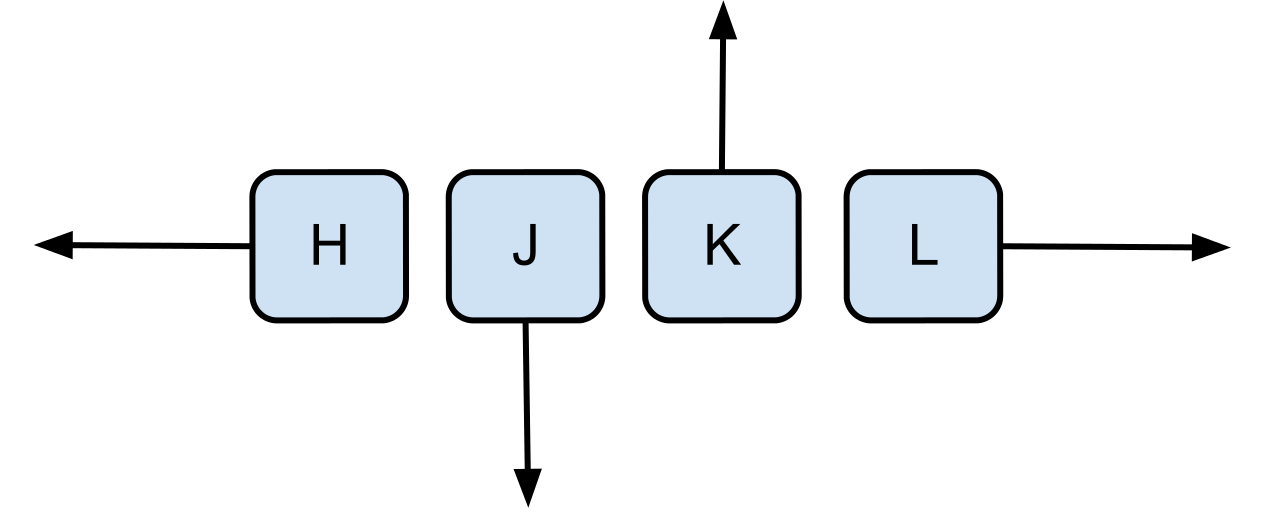
\includegraphics[width=\linewidth]{hjkl.png}
  \caption{Les «touches directionnelles» de \vim en mode normal.}
  \label{fig:vim-hjkl}
\end{figure}

Vous pouvez remarquer que ces touches sont placées sur la rangée de repos de manière à déplacer vos doigts le moins possible. En essayant de placer vos doigts pour atteindre ces lettres vous devriez vous rendre compte que l'index a deux déplacements (gauche et bas) alors que l'auriculaire n'en a pas. Vous verrez qu'on s'y fait assez rapidement et que l'index étant plus fort que l'auriculaire, ça tombe plutôt bien\footnote{Vous trouverez le clavier sur lequel \emph{Vi} a été conçu dan la section «\nameref{sec:esc}», vous comprendrez ainsi mieux pourquoi c'est comme cela.}. 

À noter qu'à force, on se sert de moins en moins des déplacements gauche/droite d'un caractère. On va leur préférer les déplacements de mot en mot, de paragraphe en paragraphe ou les déplacements grâce à des recherches.


\section{Se passer de la touche Échap}\label{sec:esc}

\section{À vous de jouer}

\TODO exercices
